\documentclass{homework}
\usepackage{cancel}
\usepackage{amsthm}
\usepackage{cleveref}
\usepackage{upgreek}
\usepackage[framed]{mcode}
\usepackage{mathrsfs}
\usepackage{tikz}
\usepackage{units}
\usetikzlibrary{matrix}
\newtheorem{lemma}{Lemma}

\title{Kevin Joyce}
\course{Math 514 - Inverse Problems}
\author{Kevin Joyce}
\docdate{\today}
\begin{document} 
\newcommand{\figref}[1]{\figurename~\ref{#1}}
\renewcommand{\bar}{\overline}
\renewcommand{\hat}{\widehat}
\renewcommand{\SS}{\mathcal S}
\newcommand{\HH}{\mathscr H}
\newcommand{\mom}{\widetilde}
\newcommand{\mle}{\widehat \Uptheta}
\newcommand{\eps}{\varepsilon}
\newcommand{\todist}{\stackrel{D}\longrightarrow}
\newcommand{\toprob}{\stackrel{p}\longrightarrow}
\newcommand{\TTheta}{\overline{\underline \Theta} }
\newcommand{\del}{\partial}
\newcommand{\approxsim}{\overset{\cdotp}{\underset{\cdotp}{\sim}}}
\begin{longproblem}
Bardsley 1.1. \emph{This problem was written in the fall of 2011 by
former University of Montana Math PhD students (and now PhD's) John
Hossler, Marylesa Howard, and Jordan Purdy:}  In baseball two
commonly collected statistics for pitchers are batting average
against (AVG) and walks plus hits per inning pitched (WHIP).
Suppose we believe that a linear relationship exists between AVG and
WHIP, and, in particular, we believe we can predict a pitcher's WHIP
from their AVG.  AVG and WHIP data for 30 Major League Baseball
(MLB) pitchers from the 2011 regular season (through September 2)
are provided in \texttt{BaseballData.m}.  Use this data to answer
the following questions.

\subproblem{ Plot AVG against WHIP such that AVG predicts WHIP. }
\begin{center}
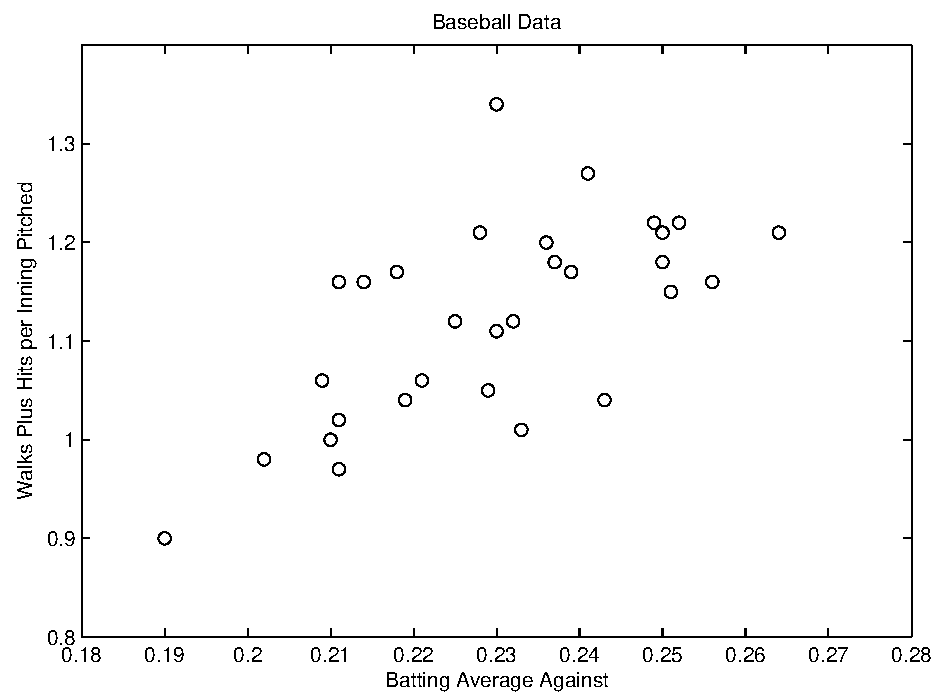
\includegraphics[width=.4\textwidth]{scatter1.pdf}
\end{center}

\subproblem{ Write out by hand the first four rows of the design matrix.  Construct the entire design matrix in MATLAB.  Include an intercept in your model. }

\begin{solution}
Let $Y_j$ be the $j$-th observed response (WHIP), $x_j$ the explanatory variable (AVG), and $\eta_i \sim N(0,\sigma^2)$ the stochastic error with some constant variance $\sigma^2$. The simple linear model is 
$$
  Y_j = \beta_0 + \beta_1 x_j + \eta_j\quad\text{ for }j=1\dots30.
$$

If we let $\vect Y,\vect x,\vect \eta$ be vectors with the given entries and $\vect \beta$ a vector with the linear coefficients, we may write the model in matrix-vector form as
$$
  \vect Y = A \vect \beta + \vect \eta,
$$
where 
$$
  A = \begin{bmatrix}
    1 &   0.209\\
    1 &   0.210\\
    1 &   0.190\\
    1 &   0.211\\
  \vdots & \vdots \\
  \end{bmatrix}
  = 
  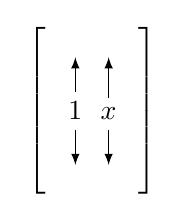
\begin{tikzpicture}[baseline=(current bounding box.center)]
  \matrix (m) [matrix of math nodes,nodes in empty cells,right delimiter={]},left delimiter={[} ]{
     &   \\
   \phantom0  &   \\
   \vect 1    & \vect x  \\
   \phantom0  &   \\
     &   \\
  };
  \draw[latex-] (m-1-1)-- (m-3-1);
  \draw[-latex] (m-3-1)-- (m-5-1);
  \draw[latex-] (m-1-2)-- (m-3-2);
  \draw[-latex] (m-3-2)-- (m-5-2);
  \end{tikzpicture}.
$$
The following MATLAB code constructs the design matrix from the given data:
\begin{verbatim}
>> A = [ones(size(AVG)) AVG]; 
\end{verbatim}
\end{solution}

\subproblem{ Compute the least squares estimate.  Note that $\vect \beta$ is a $2\times 1$ vector. }

\begin{solution}
The corresponding normal equation $A^TA \vect \beta = A^T \vect Y$ can be solved numerically with the following MATLAB command:
\begin{verbatim}
>> beta = (A'*A)\(A'*WHIP) 
 
beta =

    0.2872
    3.6386
\end{verbatim}
\end{solution}

\subproblem{ Using the model created in part (c), plot the model on the data plot from part (a).  This model predicts a pitcher's WHIP given AVG.}
\begin{center}
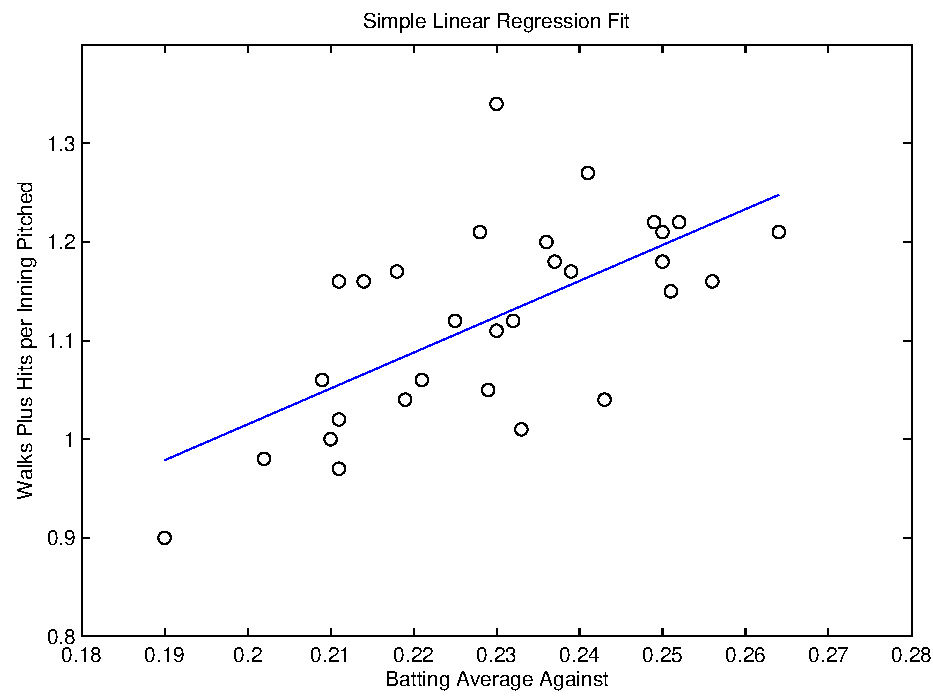
\includegraphics[width=.4\textwidth]{scatter2.pdf}
\end{center}

\subproblem{ For each observed data point, the residual is that observed value (AVG) minus the corresponding predicted value (predicted WHIP) from the model.  Calculate the thirty residuals and plot them against their corresponding AVG value.  On the same graph plot $y=0$.  Comment on whether a pattern is distinguishable or whether there is random scatter in the residual plot.  A pattern in the residuals may suggest a different model or a linear model with different error structure is more appropriate for this data set.  While random scatter does not verify our choice of this linear model is correct, it does suggest this model may be useful for analysis. }

\begin{solution}
The apparent absense of pattern in the plot on the left suggests that the model
may be useful.  Additionally, the figure on the right plots the quantiles of
the residuals versus the same quantiles of the standard normal distribution.
The ``linearity'' of these points suggests that the error structure of this
model (normal and addtive).
\begin{center}
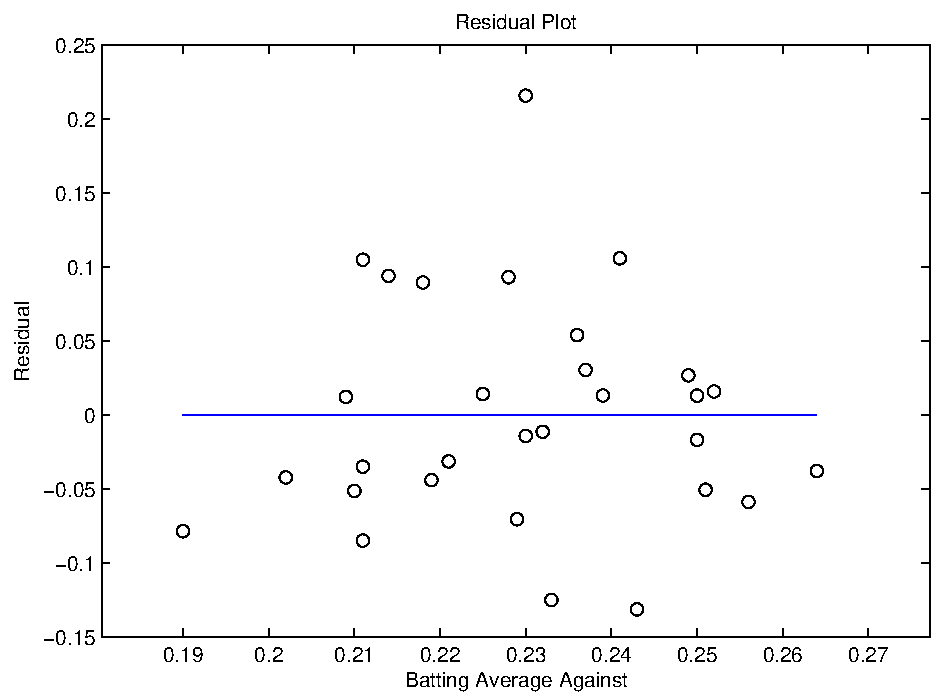
\includegraphics[width=.4\textwidth]{resid.pdf}
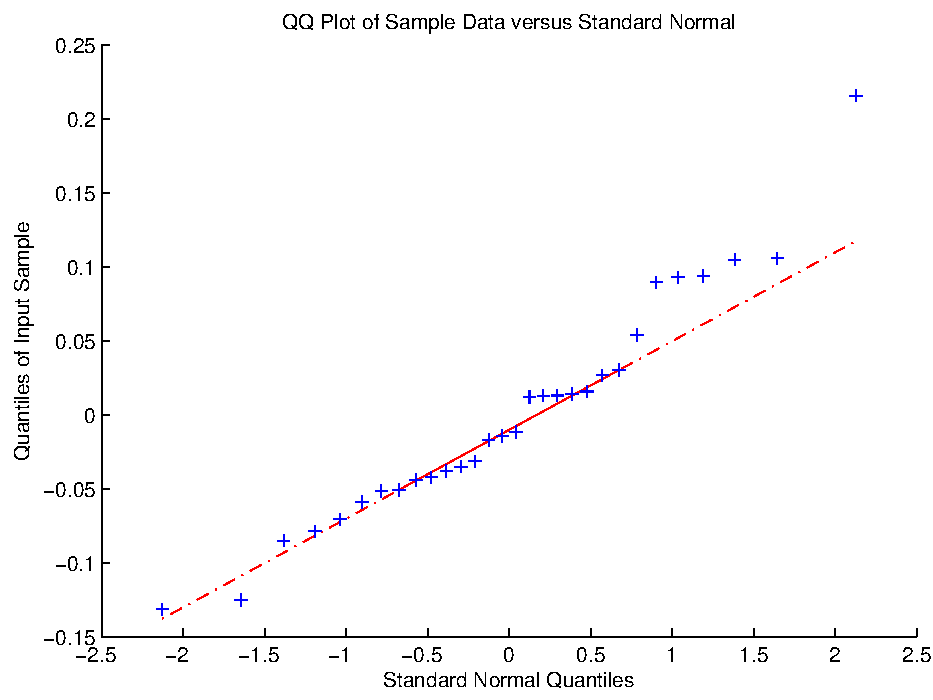
\includegraphics[width=.4\textwidth]{qqplot.pdf}
\end{center}
\end{solution}

\end{longproblem}

\begin{longproblem}
  Bardsley 1.2. The midpoint quadrature rule for a function $f$ defined on $[a,b]$ is defined by 
  \begin{equation}
    \int_a^b f(x)\,dx= (b-a)f\left(\frac{a+b}2\right) + \frac{f''(\eta)}{24}(b-a)^3,\tag{1.26}\label{midpoint}
  \end{equation}
  where $a\le\eta\le b.$

  \subproblem{ Write your own MATLAB code applying midpoint quadrature with $n=100$ grid points to approximate $\int_0^{\pi/2}\cos x\,dx=0$. }

  \begin{solution}
    We assume a uniform grid on $[0,\pi/2]$, and estimate the integral by applying (\ref{midpoint}) on each subinterval.  The following MATLAB codes implement this:
\begin{lstlisting}
n = 100;
a = 0;
b = pi/2;

s = (1/(2*n)):1/n:(1-1/(2*n)); % quadrature midpoints on unit interval
s = s*(b-a) + a; % scale to given interval
sum( cos(s)/n )
\end{lstlisting}
  \end{solution}

  \subproblem{ Determine an upper bound for the quadrature error in part (a) using (\ref{midpoint}) ($n$ times) and then verify that the inequality holds. }
  
  \begin{solution}
  Note that the second derivative of $\cos(\eta)$ is $-\cos(\eta)$, so applying (\ref{midpoint}) to each subinterval,
  $$
  \left|\int_0^{\pi/2} \cos(x)\,dx - \sum_{n=1}^{100} \cos( s_i ) \frac 1{100} \right|  =  \left|\sum_{n=1}^{100} \frac{-\cos(\eta_i)}{24}(\pi/2)^3\times 10^{-6}\right| = \sum_{n=1}^{100} \frac{\cos(\eta_i)}{24}(\pi/2)^3\times 10^{-6},
  $$
  where the last equality holds since $\cos(x) \ge 0$ for $0\le x\le\pi/2$. Note $\cos$ is decreasing on $[0,\pi/2)$, so its maximum is $\cos(a_i)$ on each subinterval where $a_i = i\pi/(2n),i=0\dots (n-1)$.  An upper bound is given by summing with $\eta_i=a_i$.  The following codes compare the actual error to the upper bound.
  \begin{lstlisting}
>> err = abs((sin(b)-sin(a)) - approx)  % Calculate error
err =

   1.0281e-05

>> err_bound = sum( cos(s-h/2) )/24e6*(pi/2)^3     % Calculate upper bound for error 

err_bound =

   1.0361e-05
\end{lstlisting}
  \end{solution}

  \subproblem{ Modify \texttt{Deblur1d.m} so that it implements midpoint quadrature on the convolution model (1.7) with kernel
  $$
  a(x) = \begin{cases}
  100s + 10,& -\frac 1{10}\le s\le 0,\\
  -100s +10,& 0\le s\le \frac 1{10},\\
  0,& \text{otherwise.}
  \end{cases}
  $$
  to obtain $\vect b = \vect A\vect x$.  Plot $a$ on $[-1,1]$.  Is the deblurring problem ill-posed with this kernel?  Support your answer. }

  \begin{solution}
  One can define $a$ as an anonymous function in MATLAB with the following code
  \begin{lstlisting}
a = @(s)( ((100*s + 10).*(s<=0) + (-100*s +10).*(s>0)).*(abs(s) < 1/10) );
  \end{lstlisting}
  The figure below is a graph of $a$ for $-1<s<1$.
  \begin{center}
  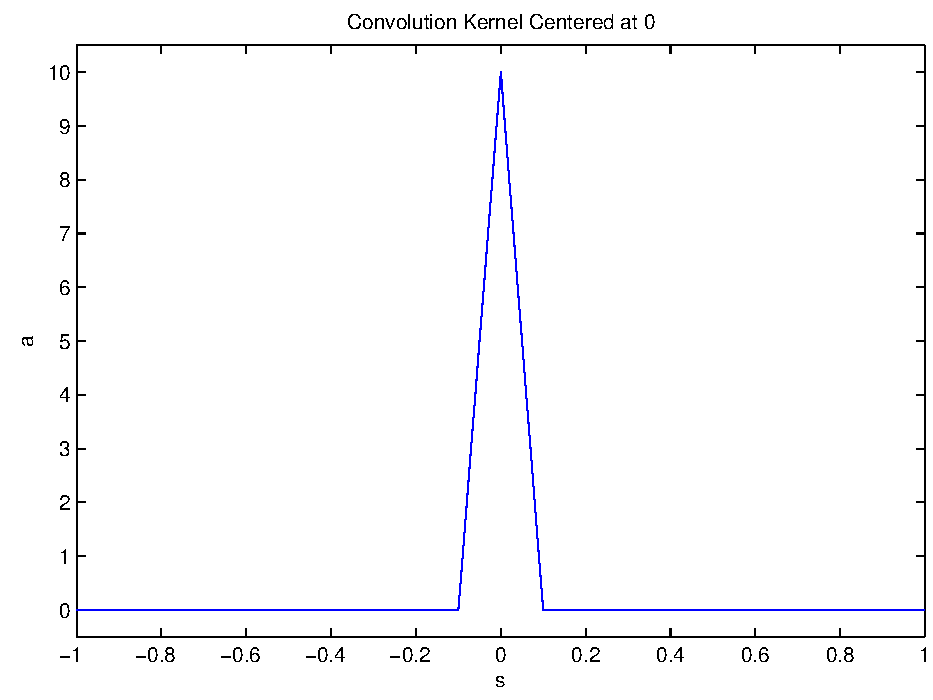
\includegraphics[width=.4\textwidth]{spike_kernel.pdf}
  \end{center}

  The deblurring problem with this kernel is also ill-posed, but less so.  The original function and blurred data points (using the kernel $a(s)$) with added Gaussian noise ($\sigma = .02$) are given in the figure on the left and the least-squares reconstruction is given in the figure to the right. 
  \begin{center}
  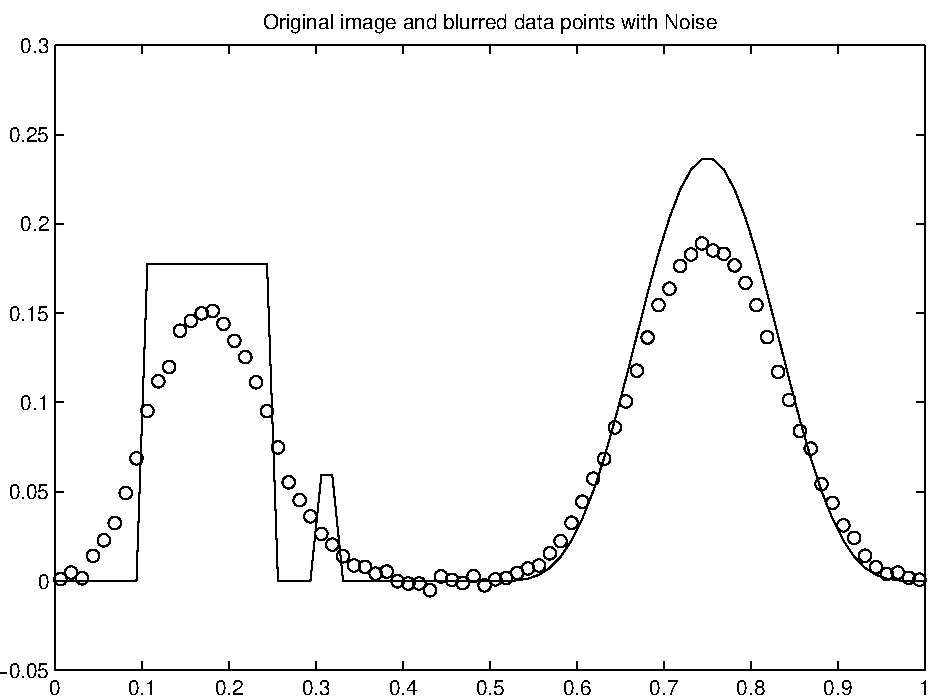
\includegraphics[width=.4\textwidth]{data.pdf}
  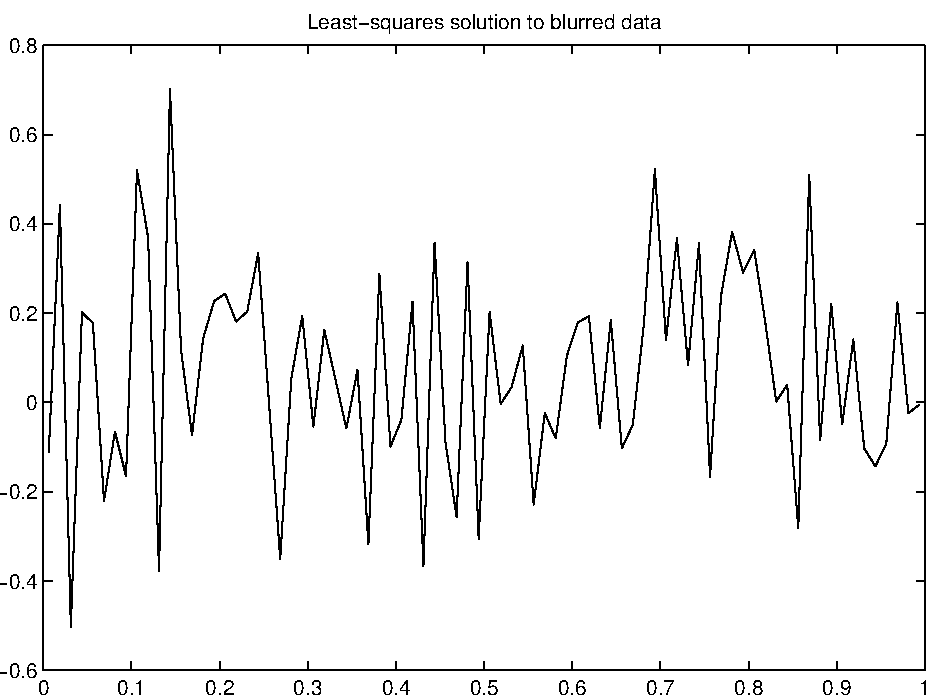
\includegraphics[width=.4\textwidth]{reconstruction.pdf}
  \end{center}
  Note that the reconstructed solution is quite poor in terms of capturing any of the characteristics of the original.  However, the magnitude of change is much less than the deblurring problem with a Gaussian kernel. The following codes indicate the magnification of the change in the solution upon deblurring.
  \begin{lstlisting}
delta_b =

    0.0188

>> delta_x 

delta_x =

    1.9031
  \end{lstlisting}

  \end{solution}
\end{longproblem}

\begin{longproblem} Bardsley 1.3.
  \subproblem{Show that 
  $$
    \vect A = \frac 1n \begin{bmatrix}
      1 & 0 & \cdots & 0\\
      1 & 1 & \ddots & 0\\
      \vdots & \vdots & \ddots & 0\\
      1 & 1 & \cdots & 1
    \end{bmatrix}_{n\times n}
  $$
 has inverse
 $$
    \vect A^{-1} = n \begin{bmatrix}
      1  & 0  & 0 & \cdots & 0\\
      -1 & 1  & \ddots & \ddots & 0\\
      0  & -1 & 1 & \ddots & 0 \\
      \vdots & \ddots & \ddots & \ddots & 0\\
      0 & \cdots & 0 & -1 & 1
    \end{bmatrix}_{n\times n}.
 $$
 Use induction on $n$.
  }

  \begin{solution}
  Note that when $n=1$, both $A$ and $A^{-1}$ are the $1\times1$ identity matrix.  The coefficients on the matricies are reciprocals, hence they are omitted in the following argument.  Now, assuming the $n$th case, let us denote the $n\times n$ matrices as $\vect A_n$ and $\vect A^{-1}_n$ (without the coefficients $n,\frac 1n$).  Note that 
  $$
  \vect A_{n+1} = \begin{bmatrix}
  \vect A_n & \vect 0_{n\times 1} \\
  \vect 1_{1\times n} & 1
  \end{bmatrix}
  \quad\text{ and }
  \quad
  \vect A_{n+1}^{-1} = \begin{bmatrix}
  \vect A_n^{-1} & \vect 0_{n\times 1}\\
  \vect x_{1\times n} & 1
  \end{bmatrix},
  $$ 
  where $\vect x_{1\times n} = \begin{bmatrix}0&\cdots&0&-1\end{bmatrix}$.  Since each matrix has compatible block decompositions, they can multiply in blocks as follows
  $$
  \vect A_{n+1} \vect A_{n+1}^{-1} = \begin{bmatrix}
  \vect A_n \vect A_n^{-1} + \vect 0_{n\times 1} \vect x_{1\times n} & \vect A_n \vect 0_{n\times 1} + \vect 0_{n\times 1} 1 \\
  \vect 1_{1\times n} \vect A_n^{-1} + 1\vect x_{1\times n} & \vect 1_{1\times n} \vect 0_{n\times 1} + 1
  \end{bmatrix}
  =\begin{bmatrix}
  \vect I_{n\times n} & \vect 0_{n\times 1}\\
  \vect -\vect x_{1\times n} + \vect x_{1\times n} & 1
  \end{bmatrix},
  $$
  and
  $$
    \vect A_{n+1}^{-1} \vect A_{n+1} = \begin{bmatrix}
  \vect A_n^{-1}\vect A_n  + \vect 0_{n\times 1} \vect 1_{1\times n} & \vect A_n \vect 0_{n\times 1} + \vect 0_{n\times 1} 1 \\
  \vect x_{1\times n}\vect A_n + 1\vect 1_{1\times n} & \vect x_{1\times n}\vect 0_{n\times 1} + 1
  \end{bmatrix}
  =\begin{bmatrix}
  \vect I_{n\times n} & \vect 0_{n\times 1}\\
  \vect -\vect 1_{1\times n} + \vect 1_{1\times n} & 1
    \end{bmatrix}.
  $$
  \end{solution}

  \subproblem{Show that $\vect A^{-1}$ corresponds to the discritization of $\frac d{ds}$  on the grid $\{s_j'\}_{j=1}^n$, where $s_j' = (j-\frac 12)/n$, with a zero Dirichlet boundary condition on the left (i.e. $x(s_0') = 0$) and a zero Neumann boundary condition on the right (i.e. $s_{n+1}' = s_n'$).  Use the forward difference approximation of the derivative:
  $$
    \frac d{ds} x(s_j') \approx \frac{ x(s_j') - x(s_{j-1}')}{h}.
  $$
  }

  \begin{solution}
  The columns of the linear operator defined above are given by how it operates on the standard basis vectors.  I.e. $\vect a_j = \frac d{ds} \vect e_j$ where $\vect a_j$ is the $j$th column of the matrix representation and $\vect e_j$ is the vector with 1 in the $j$th coordinate and 0 elsewhere.  For the case of $0\le j \le n$, note that $a_{jj} = (1 - 0)/h$, $a_{j+1,j} = (0 - 1)/h$ and $(0 - 0)/h = 0$ otherwise.

  Note that with the Neumann condition, we can extend the operator to $\tilde A:\RR \to \RR^{n+1}$ where $[\tilde A x](s_{n+1}) = \frac 1h \cdot (x(s_n) - x(s_{n+1})) \equiv 0$.  Hence the final row must have each coordinate be $0$.
  \end{solution}

  \subproblem{ Replace $\vect A$ by $\vect A^{-1}$ in \texttt{PSFrecon.m}.  How do the results change?  Is $b = \vect A^{-1}\vect x$ an illposed problem, i.e. does it fail any of the three conditions of Definition 1.1? }

  \begin{solution}
  In this case, we are inverting the discrete derivative by backward differencing which results multiplication by $\vect A$.  Because this inverse exists, both existence and uniqueness are guaranteed. However, there appears to be little sensitivity to changes in the data, as evidenced by the following reconstruction.
  \begin{center}
  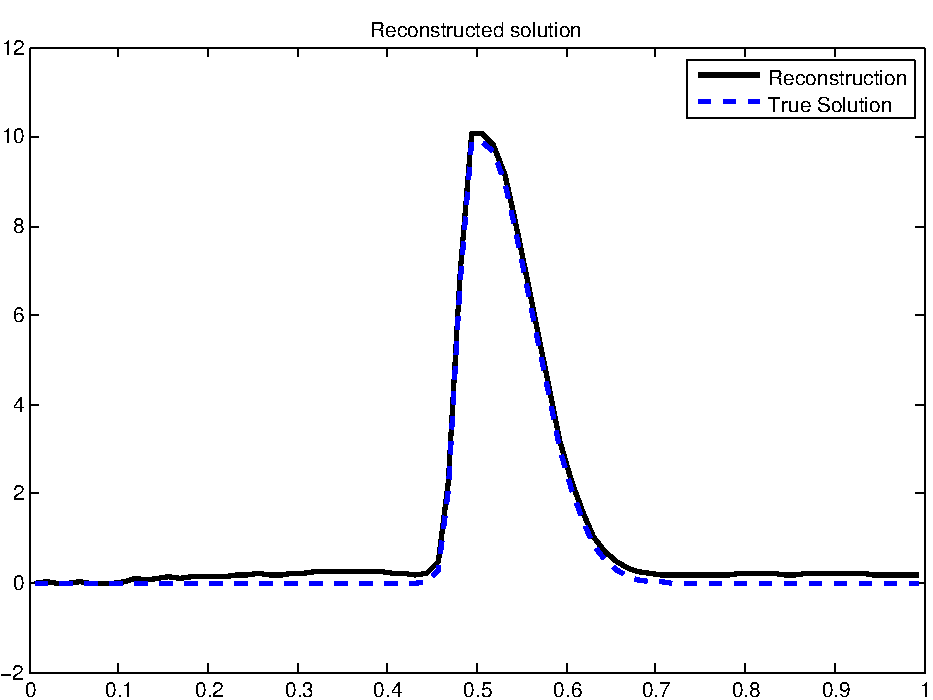
\includegraphics[width=.4\textwidth]{nonillposed.pdf}
  \end{center}
  
  Note that multiplication by $\vect A$ is numerically integrating the diffential equation $x' = d$ using something similar to Euler's method, which is known to be reasonably stable.  Moreover, note that the columns of $\vect A$ are orthogonal.
  \end{solution}

\end{longproblem}

\begin{longproblem} Bardsley 1.5. Define
\renewcommand{\arraystretch}{1.5}
$$
  \vect A = \begin{bmatrix}
  1 & 1\\
  1 & 0\\
  0 & 1\\
  \end{bmatrix}.
$$
\end{longproblem}

\subproblem{Compute the singular value decomposition of $\vect A$ by hand: $\vect A = \vect U \vect \Sigma \vect V^T$, where $\vect U\in \RR^{3\times 3}$ is orthogonal and $\vect \Sigma \in \RR^{3\times 2}$ is diagonal, and $\vect V\in \RR^{2\times 2}$ is orthogonal.}
\newpage
\mbox{}
\newpage

\subproblem{Using the columns of $\vect U$ and $\vect V$ as basis elements write down bases for the four subspaces: the column space $C(\vect A)$, the row space $C(\vect A^T)$, the nullspace $N(\vect A)$, and the left null space $N(\vect A^T)$.}

\begin{solution}
  Let $\vect A \in \RR^{m\times n}$ have a singular value decomposition $\vect A=\vect U\vect \Sigma \vect V^T$ and $k$ be the index of the first \emph{positive} singular value.  For $\vect x \in \RR^m$,  
  $$
    \vect A\vect x = \sum_{i=k}^{\min\{n,m\}} \left(\sigma_i [\vect V^* \vect x]_i\right) \, \vect u_i,
  $$
  and since each $u_i$ are mutually orthogonal non-zero vectors, the subset
  $\{\vect u_k,\dots,\vect u_{\min \{m,n\}}\}$ forms a basis for the range $C(\vect A)$.  
  Since $\vect A^T = \vect V\vect \Sigma^T \vect U^T$, 
  A similar argument shows the vectors 
  $\{\vect v_k,\dots,\vect v_{\min \{m,n\}}\}$ form a basis for $C(\vect A^T)$.

  Note that $\vect A\vect x = 0$ if $\vect x = \{\vect v_1,\dots, \vect
  v_{k-1}, \vect v_{\min\{n,m\}+1},\dots,\vect v_{\max\{n,m\}}\}$.  By the
  Rank-Nullity theorem, these vectors suffice for making up a basis for all of
  $N(\vect A)$.  Similarly, $\vect x = \{\vect u_1,\dots, \vect
  u_{k-1}, \vect u_{\min\{n,m\}+1},\dots,\vect u_{\max\{n,m\}}\}$ makes up a basis of $N(\vect A^T)$.
\end{solution}

\subproblem{Using the SVD computed in (a), compute the psuedo-inverse $\vect A^\dagger$ of $\vect A$, and then use it to compute the least squares solution $\vect x_{\mathrm{LS}}=\vect A^\dagger b$ of 
\renewcommand{\arraystretch}{1.5}
$$
  \begin{bmatrix}
  1 & 1\\
  1 & 0\\
  0 & 1\\
  \end{bmatrix}
  \begin{bmatrix}
    x_1\\
    x_2\\
  \end{bmatrix}
  =
  \begin{bmatrix}
    1\\
    1\\
    1\\
  \end{bmatrix}
$$}

\begin{solution}
\renewcommand{\arraystretch}{2}
Note that $\vect \Sigma^\dagger$ is given by the $n\times m$ matrix with $\sigma_i^{-1}$ on the main diagonal.  So, from the above calculations
\begin{align*}
  \vect A^\dagger &= \vect V \vect \Sigma^\dagger \vect U^T \\
  &=\frac 1{\sqrt{2}} 
  \begin{bmatrix} 1 & 1\\ -1 & 1 \end{bmatrix}
  \begin{bmatrix} 1 & 0 & 0 \\ 0 & \frac 1{\sqrt{3}} & 0\end{bmatrix}
  \begin{bmatrix} 
    0 & \frac 1{\sqrt2} & -\frac 1{\sqrt2}\\ 
    \sqrt{\frac 23} & \frac 1{\sqrt6} & \frac1{\sqrt6}\\
    -\frac1{\sqrt3} & \frac1{\sqrt3} & \frac1{\sqrt3}
  \end{bmatrix}\\
  &=
  \frac 13 \begin{bmatrix}
  1 & 2 & -1\\
  1 & -1 & 2
  \end{bmatrix}
\end{align*}
Hence, $\vect x_{\mathrm{LS}}$ is given by
\renewcommand{\arraystretch}{1.5}
$$
\vect A^\dagger
   \begin{bmatrix}
    1\\
    1\\
    1\\
  \end{bmatrix}
  =
  \frac 13 \begin{bmatrix}
  1 & 2 & -1\\
  1 & -1 & 2
  \end{bmatrix}
   \begin{bmatrix}
    1\\
    1\\
    1\\
  \end{bmatrix}
  =\begin{bmatrix} \frac23 \\ \frac 23\end{bmatrix}
$$

\end{solution}

\subproblem{Compare the solutions in (c) with the solution to the normal
equations, $\vect A^T\vect A\vect x =\nolinebreak \vect A^T\vect b$. The two solutions
should agree.}

\begin{solution}
Note the MATLAB output numerically solves the normal equation which agrees with the analysis above:
\begin{lstlisting}
>> A = [1 1; 1 0; 0 1]; b = [1 1 1]'; 
>> A\b  
 
ans =
                                                                                                                                            
    0.6667                                                                                                                                  
    0.6667                                                                                                                                  
                                                                                                                                            
>>                                                                                                                                          
\end{lstlisting}
\end{solution}

\end{document} 
